\documentclass[a4paper,12pt]{scrartcl}
\usepackage[left= 2.5cm,right = 2cm, bottom = 4 cm, top = 2.5cm]{geometry}
\usepackage[utf8x]{inputenc}
\usepackage {graphicx}
\usepackage[ngerman]{babel}

\begin{document}
\section{Daten}
\label{sec:daten}
In diesem Abschnitt wird gezeigt was für Daten für den Öffentlichen Verkehr(https://opentransportdata.swiss) zur Verfügung stehen. Anschliessend werden die Datenformate vorgestellt und analysiert. Die Fahrplandaten werden in zwei verschiedenen Formaten bereitgestellt GTFS und HRDF. 

\subsection{Fahrplan General Transit Feed Specification (GTFS)}
\label{sec:gtfs-static}
General Transit Feed Specification (GTFS) ist ein von Google entwickeltes Dateiformat zum Austausch von Öffentlichen Verkehrsdaten sprich Fahrpläne. Ursprünglich wurde es Google Transit Feed Specification (GTFS) genannt (bis 2010), weil es ausschliesslich für Google Maps genutzt wurde. Dies änderte sich aber mit der Zeit sehr stark da viele neue Applikationen herauskamen die diese Daten verwendeten die nicht von Google waren und somit änderte man den Namen zu General Transit Feed Specification (GTFS).
%http://gtfs.org/gtfs-background/

GTFS beinhaltet nicht nur Informationen über Fahrpläne sondern auch über Geographische Orte wie Haltestellen. GTFS ist ein statisches Dateiformat und beinhaltet keine Echtzeitdaten deshalb wird es auch GTFS Static genannt. 

\subsubsection{Datenstruktur}
\label{sec:gtfs-datenstruktur}
Die GTFS Datei besteht aus nichts anderen als Textfiles, die durch Datenfelder(Werte) und Kommas getrennt sind, dieses Format nennt man auch Comma-Separated Values (CSV).
%https://tools.ietf.org/html/rfc4180
\begin{figure}[]
	\centering
	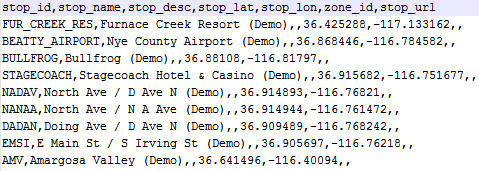
\includegraphics[width=8cm]{img/bspcsv.png}
	\caption{Dateiformat CSV}
	\label{fig:gtfs-dateiformat}
\end{figure}

Die verschiedenen Textfiles decken viele wichtige Informationen ab, die für ein GTFS benötigt werden.
 \begin{figure}[]
 	\includegraphics[width=14cm]{img/inhalt.png}
 	\caption{Inhalt eines GTFS \cite{gtfsInhalt}}
 	\label{fig:gtfs-inhalt}
 \end{figure}
 \cite{Inhalt}
%https://developers.google.com/transit/gtfs/reference/
\begin{figure}[]
	\centering
	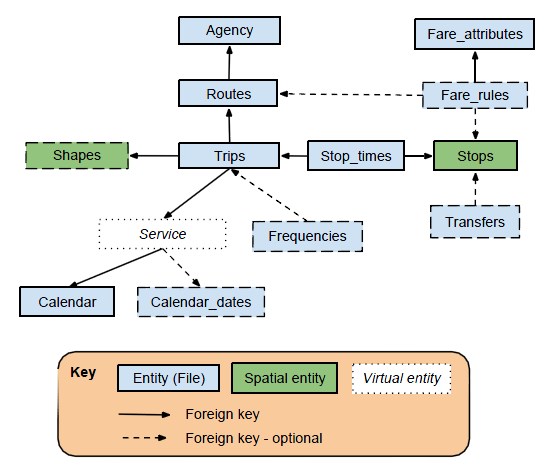
\includegraphics[scale=0.75]{img/GTFS_data_model_diagram.png}
 	\caption{Uebersicht \cite{gtfsUebersicht}}
	\label{fig:gtfs-uebersicht}
\end{figure}
%https://www.transitwiki.org/TransitWiki/images/f/ff/GTFS_data_model_diagram.PNG
 

\subsubsection{Vor- und Nachteile}
\label{sec:gtfs-vornachteile}
Die Daten können einfach von Mensch und Maschine gelesen werden, wegen dem einfachen Aufbau der Textfiles. Zudem sind stellt Google hierfür eine sehr gute Anleitung zur Verfügung wie diese Daten verwendet werden und aufgebaut sind.

\subsection{GTFS Realtime (GTFS-RT)}
\label{sec:gtfs-rt}
GTFS-RT ist eine Erweiterung der GTFS-Static Daten. Wie der Name Realtime schon sagt handelt sich hier um Echtzeitdaten. 
\subsubsection{Datenstruktur}
\label{sec:gtfs-rt-datenstruktur}
GTFS-RT stellt folgende Daten zusätzlich in diesem Format zur Verfügung. Die Daten werden geschrieben/gelesen basierend auf sogenannten "Protocol Buffers", die stehen in vielen Programmiersprachen zur Verfügung (C++,C, Go, Java, Python).
\begin{itemize}
	\item{\textbf{Trip Updates}} -Hier werden Aktuelle Verspätungen, geänderte Routen, Ersatzfahrzeuge oder Ausfälle publiziert.  
	\item{\textbf{Service Alerts}} -Hier werden Informationen über Probleme mit Stationen,  Linien, das Ganze Netzwerk etc. übermittelt. 
	\item{\textbf{Vehicle Positions}} -Hier werden Daten geliefert die eine genaue Position des Vehicles mit der dazugehörigen Zeit liefert. 
\end{itemize}
%https://opentransportdata.swiss/de/cookbook/gtfs-rt/
%https://developers.google.com/transit/gtfs-realtime/guides/feed-entities
\subsubsection{Vor- und Nachteile}
\label{sec:gtfs-rt-vornachteile}
Google stellt auch hier eine Gute Übersichtliche Anleitung zur Verwendung von GTFS-RT zur Verfügung.

\subsection{Fahrplan Hafas Rohdaten Format (HRDF)}
\label{subsec:hrdf}
Neben GTFS ist HRDF ein weiteres Dateiformat das die Fahrplandaten zur Verfügung stellt. 
Dieses Dateiformat kommt von der Firma HaCon. Das Format wird für ihren eigenen Journey Planner (HaCon Fahrplan-Auskunfts-System (HAFAS)) genutzt. Zudem stellt HaCon eine Plannungssoftware (Train Planning System TPS) für Infrastrukturbetreiber (wie Eisenbahnverkehrsunternehmen usw.) zur Verfügung. HRDF ist somit ihr eigenes Datenaustauschformat von Fahrplandaten.




%http://www.hacon.de/tps

%http://www.hacon.de/hafas/daten

\begin{figure}[]
	\centering
	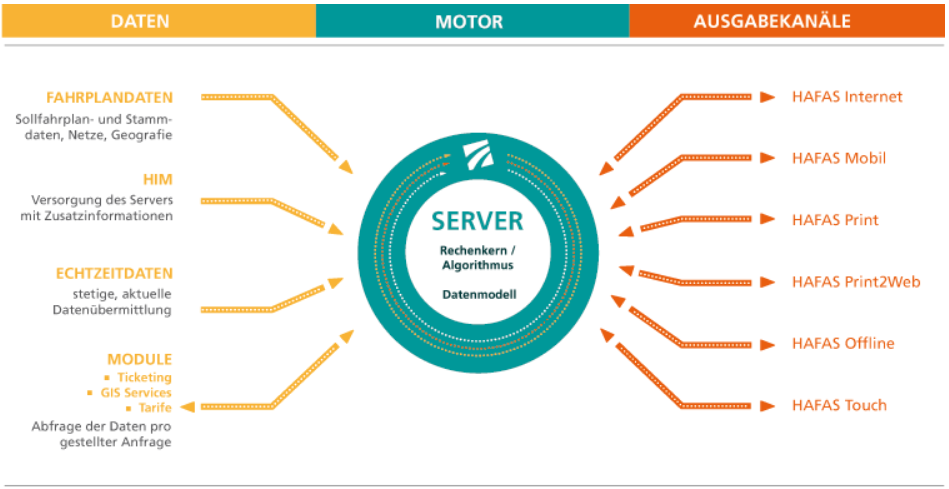
\includegraphics[scale=0.75]{img/HAFAS.png}
	\caption{Uebersicht HAFAS \cite{haconUebersicht}}
	\label{fig:hafas-uebersicht}
\end{figure}



\subsubsection{Datenstruktur}
\label{sec:hrdf-datenstrukur}
Ähnlich wie GTFS files sind auch HRDF Files auch Textfiles aber mit dem unterschied das die Werte im Stil Tab-separated values (TSV) angelegt sind. Die Daten sind auch anders aufgebaut.
Nebenbei können HRDF Daten auch in GTFS-Daten konvertiert werden.
\begin{figure}[]
	\centering
	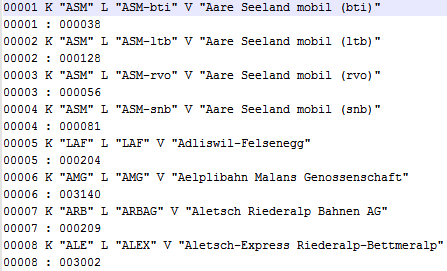
\includegraphics[width=8cm]{img/bsptsv.png}
	\caption{Dateiformat TSV}
	\label{fig:hrdf-dateiformat}
\end{figure}


%http://gtfs.geops.ch/doc/   HRDF->GTFS konvertieren
%INFO+ HRDF-Exportschnittstelle
%https://opentransportdata.swiss/content/uploads/2016/10/hrdf.pdf
\subsubsection{Vor- und Nachteile}	
\label{sec:hrdf-vornachteile}
HRDF ist nicht so gut dokumentiert. Opentransportdata.swiss, die Daten zur Verfügung stellt warnt zudem noch: "Die HRDF-Datei(en) sind relativ komplex. Ohne Not sollte nicht damit gearbeitet werden."\cite{opentransporthrdf}
%https://opentransportdata.swiss/de/cookbook/hafas-rohdaten-format-hrdf/


\subsection{Dienststellendokumentation (DiDok)}
\label{sec:didok}
Bei dieser Dokumentation geht es um die Daten zur Verwaltung der Stammdaten aller Dienststellen(Haltestellen) des öffentlichen Verkehrs der Schweiz. In dem Format werden Daten wie offizieller Name einer Haltestelle und die dazugehörige verantwortliche Geschäftsorganisation. Es werden aber auch die geographischen Koordinaten der Haltestellen mitgeliefert. Die Datei wird im Excel Format zur Verfügung gestellt.

\begin{figure}[]
	\centering
	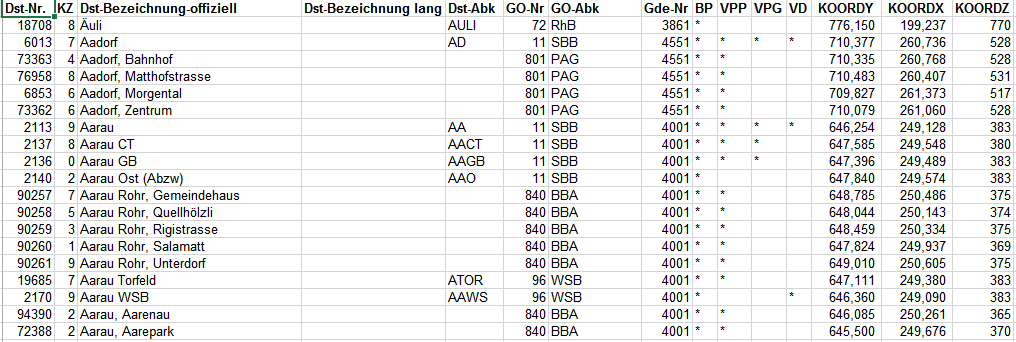
\includegraphics[width=17cm]{img/didokdateiformat.png}
	\caption{DiDok Dateiformat}
	\label{fig:didok-dateiformat}
\end{figure}

\begin{figure}[]
	\centering
	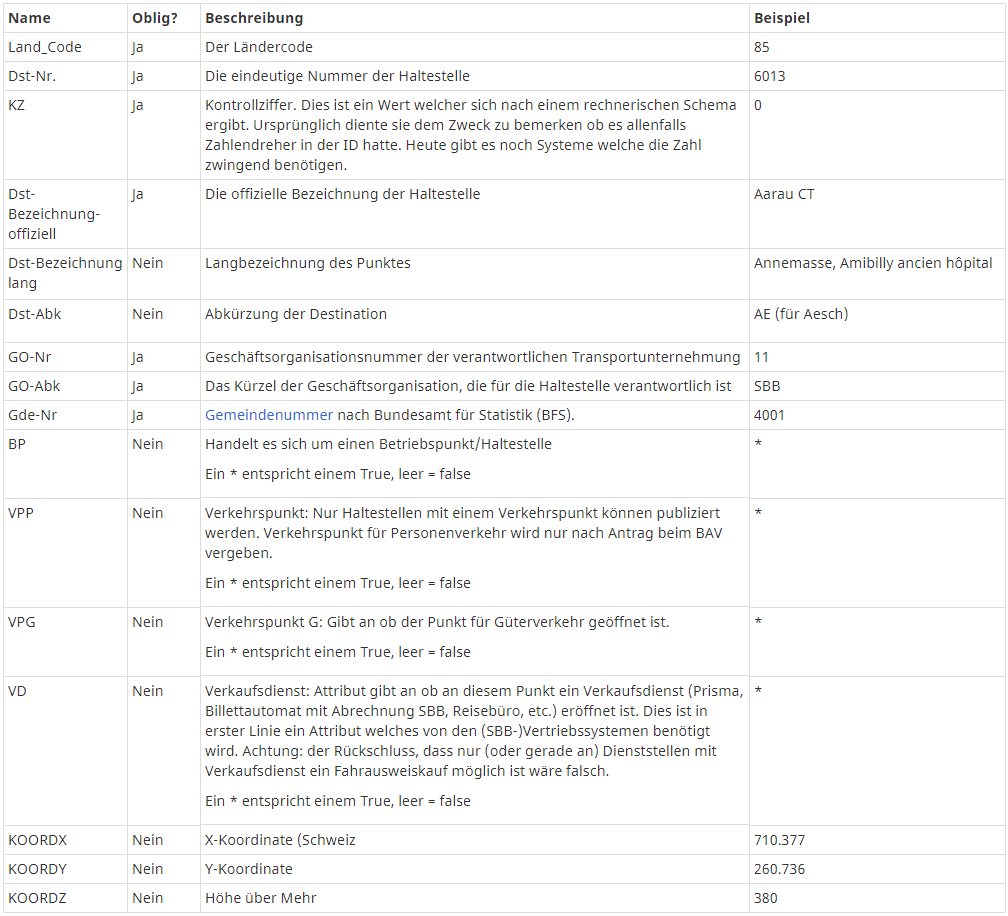
\includegraphics[scale=0.75]{img/didokuebersicht.png}
	\caption{DiDok Übersicht  \cite{didok}}
	\label{fig:didok-uebersicht}
\end{figure}


\subsection{Ist-Daten (actual data)}
\label{sec:istdaten}
Bei den Ist-Daten handelt es sich um eine Ansammlung von Daten, welche die effektive gefahrenen Fahrten des letzten Tages enthalten. Somit sind diese Daten eigentlich in dem Sinne keine wirklichen Ist-Daten. Diese Daten können aber durchaus interessant sein für Statistiken:\cite{istdaten}
\begin{itemize}
	\item{Pünktlichkeit}   
	\item{Regelmässigkeit}. 
	\item{Anschlussqualität}  
\end{itemize}
Die Daten werden als CSV-Datei bereitgestellt.

\subsection{Fahrplan Überblick (timetable overview)}


\subsection{Fahrtprognose (trip forecast)}


\subsection{Abfahrts-/Ankunftsanzeiger (departure/arrival display)}




\end{document}